\sectionlink{1ループ振幅}\label{ch:7}

関係する曲面を記述した後、トーラスに焦点を当て、まずこの曲面上の CFT を、次いで弦の振幅を調べる。その後、開弦理論および向き付けのない理論へ一般化する。理解すべき最も重要な問題は、短距離（UV）発散が存在しないことである。

\subsectionlink{Riemann面}

Euler 数がゼロの Riemann面は四つある。

\subsubsectionlink*{トーラス}

第5.1節で議論したトーラス $T^2$ は、Euler 数がゼロである唯一の閉じた向き付けのある曲面である。計量 $ds^2=dw\,d\bar w$ を持つ複素平面に、同一視
\begin{equation}
w\cong w+2\pi\cong w+2\pi\tau
\tag{7.1.1}\label{eq:7.1.1}
\end{equation}
を課して記述する。モジュライは $\tau=\tau_1+i\tau_2$ の実部と虚部の二つ、CKV は平行移動を表す二つである。実座標 $w=\sigma^1+i\sigma^2$ で書けば、
\begin{equation}
(\sigma^1,\sigma^2)\cong(\sigma^1+2\pi,\sigma^2)
\cong(\sigma^1+2\pi\tau_1,\sigma^2+2\pi\tau_2)
\tag{7.1.2}\label{eq:7.1.2}
\end{equation}
となるので、トーラスは、周長 $2\pi$、長さ $2\pi\tau_2$ の円筒の両端を、角度 $2\pi\tau_1$ だけ回転させてから縫い合わせたものと考えられる。

座標 $z=\exp(-iw)$ を用いると、同一視 $w\cong w+2\pi$ は自動的に満たされ、$w\cong w+2\pi\tau$ は
\begin{equation}
z\cong z\exp(-2\pi i\tau)
\tag{7.1.3}\label{eq:7.1.3}
\end{equation}
となる。一つの基本領域は環状領域
\begin{equation}
1\leq |z|\leq\exp(2\pi\tau_2)
\tag{7.1.4}\label{eq:7.1.4}
\end{equation}
である。外側の円を $2\pi\tau_1$ 回転させ、内側と外側の円を縫い合わせるとトーラスになる。特に断らない限り、$w$ 座標を用いる。

\subsubsectionlink*{円筒（環帯）}

円筒 $C_2$ は領域
\begin{equation}
0\leq\operatorname{Re}w\leq\pi,\qquad w\cong w+2\pi it
\tag{7.1.5}\label{eq:7.1.5}
\end{equation}
である。すなわち、幅 $\pi$、長さ $2\pi t$ の帯の両端をつないだものである。モジュラスは $t$ 一つで、$0<t<\infty$ の全範囲を動く。トーラスとは異なり、モジュラー群は存在せず、長い円筒の極限 $t\to0$ は、長い帯の極限 $t\to\infty$ と大きく異なる。CKV は、境界に平行な平行移動一つである。

円筒は、純虚数の $\tau=it$ を持つトーラスに、対合
\begin{equation}
w'=-\bar w
\tag{7.1.6}\label{eq:7.1.6}
\end{equation}
による同一視を施して得られる。これは虚軸に関する反射である。直線 $\sigma^1=0,\pi$ はこの反射で固定されるため、境界になる。他方の座標は周期的に同一視される。
\begin{equation}
(\sigma^1,0)\cong(\sigma^1,2\pi t).
\tag{7.1.7}\label{eq:7.1.7}
\end{equation}

\subsubsectionlink*{Klein の壺}

Klein の壺 $K_2$ は、複素平面に同一視
\begin{equation}
w\cong w+2\pi\cong-\bar w+2\pi it
\tag{7.1.8}\label{eq:7.1.8}
\end{equation}
を課したもの、あるいは
\begin{equation}
(\sigma^1,\sigma^2)\cong(\sigma^1+2\pi,\sigma^2)
\cong(-\sigma^1,\sigma^2+2\pi t)
\tag{7.1.9}\label{eq:7.1.9}
\end{equation}
とみなせる。これは周長 $2\pi$、長さ $2\pi t$ の円筒の両端を、パリティ反転 $\Omega$ の後に縫い合わせたものである。唯一のモジュラス $t$ は $0<t<\infty$ を動き、モジュラー群は存在しない。唯一の CKV は $\sigma^2$ 方向の平行移動である。Klein の壺は、モジュラス $\tau=2it$ のトーラスに
\begin{equation}
w'=-\bar w+2\pi it
\tag{7.1.10}\label{eq:7.1.10}
\end{equation}
による同一視を施して得られる。Klein の壺は、二つのクロスキャップを付けた球面とも考えられるが、この記述は第7.4節まで先送りする。

\subsubsectionlink*{Möbius の帯}

Möbius の帯 $M_2$ は、帯を $\Omega$ によってひねって縫い合わせたものである。
\begin{equation}
0\leq\operatorname{Re}w\leq\pi,\qquad
w\cong-\bar w+\pi+2\pi it.
\tag{7.1.11}\label{eq:7.1.11}
\end{equation}
ここでもモジュラス $t$ は $0<t<\infty$ を動き、唯一の CKV は $\sigma^2$ 方向の平行移動である。$\tau=2it$ のトーラスに、二つの対合
\begin{equation}
w'=-\bar w,\qquad w'=w+\pi(2it+1)
\tag{7.1.12}\label{eq:7.1.12}
\end{equation}
による同一視を施して得られる。Möbius の帯は、クロスキャップを一つ付けた円板とも考えられるが、この記述も後に回す。

\subsectionlink{トーラス上のCFT}

\subsubsectionlink*{スカラーの相関関数}

球面の場合と同じく、Green 関数(6.2.7)から出発する。これは
\begin{equation}
\frac{2}{\alpha'}\bar\partial\partial
G'(w,\bar w;w',\bar w')
=-2\pi\delta^2(w-w')+\frac{1}{4\pi\tau_2}
\tag{7.2.1}\label{eq:7.2.1}
\end{equation}
を満たす。Green 関数はトーラス上の両方向について周期的であり、源と背景電荷の項を除けば、正則関数と反正則関数の和になる。これらの性質から、これはテータ関数に関係するものとわかる。テータ関数の性質は本節の末尾にまとめる。具体的には、
\begin{equation}
G'(w,\bar w;w',\bar w')
\sim-\frac{\alpha'}{2}
\ln\left|\vartheta_1\left(\left.\frac{w-w'}{2\pi}\right|\tau\right)\right|^2
\tag{7.2.2}\label{eq:7.2.2}
\end{equation}
と推測する。関数 $\vartheta_1$ は第一引数がゼロに近づくと線形に消え、$w\to w'$ における正しい振る舞いを与える。それ以外の場所では、対数は正則関数と反正則関数の和であるため、$\bar\partial\partial$ で消える。しかし、準周期性\hyperref[eq:7.2.32b]{(7.2.32b)}のため、この関数は完全には二重周期的でない。$w\to w+2\pi\tau$ のもとで $-\alpha'[\operatorname{Im}(w-w')+\pi\tau_2]$ だけ変化する。また、背景電荷も欠けている。両方とも容易に修正できる。
\begin{equation}
\begin{aligned}
G'(w,\bar w;w',\bar w')
={}&-\frac{\alpha'}{2}
\ln\left|\vartheta_1\left(\left.\frac{w-w'}{2\pi}\right|\tau\right)\right|^2\\
&+\alpha'\frac{[\operatorname{Im}(w-w')]^2}{4\pi\tau_2}
+k(\tau,\bar\tau).
\end{aligned}
\tag{7.2.3}\label{eq:7.2.3}
\end{equation}
関数 $k(\tau,\bar\tau)$ は $X_0$ との直交性によって定まるが、球面の場合と同じく、時空の運動量保存により結果から消える。

頂点演算子の積の期待値は、球面上で先に得た結果(6.2.13)と同様に、
\begin{equation}
\begin{aligned}
\left\langle\prod_{i=1}^{n}
{:}e^{ik_i\cdot X(z_i,\bar z_i)}{:}\right\rangle_{T^2}
={}&iC_{T^2}^{X}(\tau)(2\pi)^d\delta^d\left(\sum_i k_i\right)\\
&\times\prod_{i<j}\left|
\frac{2\pi}{\partial_\nu\vartheta_1(0|\tau)}
\vartheta_1\left(\left.\frac{w_{ij}}{2\pi}\right|\tau\right)
\exp\left[-\frac{(\operatorname{Im}w_{ij})^2}{4\pi\tau_2}\right]
\right|^{\alpha'k_i\cdot k_j}
\end{aligned}
\tag{7.2.4}\label{eq:7.2.4}
\end{equation}
で与えられる。因子 $2\pi/\partial_\nu\vartheta_1$ は、繰り込まれた自己縮約から生じる。

\subsubsectionlink*{スカラーの分配関数}

球面の全体の規格化は弦の結合定数に吸収したが、トーラスではそうすることはできない。特に、非自明な $\tau$ 依存性があるからである。実際、頂点演算子をまったく含まない振幅にも、多くの物理があることがわかる。頂点演算子のない経路積分 $\langle1\rangle_{T^2(\tau)}\equiv Z(\tau)$ を考えよう。モジュラス $\tau$ のトーラスは、円周上の場の理論をとり、Euclid 時間 $2\pi\tau_2$ だけ発展させ、$\sigma^1$ 方向に $2\pi\tau_1$ 平行移動し、それから両端を同一視することで形成されると考えられる。演算子の言葉では、これはトレース
\begin{equation}
\begin{aligned}
Z(\tau)&=\operatorname{Tr}\left[\exp(2\pi i\tau_1P-2\pi\tau_2H)\right]\\
&=(q\bar q)^{-d/24}\operatorname{Tr}\left(q^{L_0}\bar q^{\tilde L_0}\right)
\end{aligned}
\tag{7.2.5}\label{eq:7.2.5}
\end{equation}
を与える。ここで $q=\exp(2\pi i\tau)$ である。運動量 $P=L_0-\tilde L_0$ は $\sigma^1$ の平行移動を生成し、Hamiltonian $H=L_0+\tilde L_0-\tfrac1{24}(c+\tilde c)$ は、式(2.6.10)のように $\sigma^2$ の平行移動を生成する。Hamiltonian と他の保存量の指数関数で重みを付けたこのようなトレースは、統計力学と同じく分配関数と呼ばれる。

トレースは、各 $\mu,n$ に対する占有数 $N_{\mu n},\tilde N_{\mu n}$ についての和と、運動量 $k^\mu$ についての積分に分かれる。Virasoro 生成子も同様に和に分かれ、$Z(\tau)$ は
\begin{equation}
V_d(q\bar q)^{-d/24}\int\frac{d^dk}{(2\pi)^d}
\exp(-\pi\tau_2\alpha'k^2)
\prod_{\mu,n}\sum_{N_{\mu n},\tilde N_{\mu n}=0}^{\infty}
q^{nN_{\mu n}}\bar q^{n\tilde N_{\mu n}}
\tag{7.2.6}\label{eq:7.2.6}
\end{equation}
となる。時空体積 $V_d$ の因子は、運動量の連続体での規格化、すなわち $\sum_k$ が $V_d(2\pi)^{-d}\int d^dk$ になることから生じる。それぞれの和は等比級数であり、
\begin{equation}
\sum_{N=0}^{\infty}q^{nN}=(1-q^n)^{-1}
\tag{7.2.7}\label{eq:7.2.7}
\end{equation}
なので、
\begin{equation}
Z(\tau)=iV_dZ_X(\tau)^d
\tag{7.2.8}\label{eq:7.2.8}
\end{equation}
を得る。ここで
\begin{equation}
Z_X(\tau)=(4\pi^2\alpha'\tau_2)^{-1/2}|\eta(\tau)|^{-2}.
\tag{7.2.9}\label{eq:7.2.9}
\end{equation}
また、
\begin{equation}
\eta(\tau)=q^{1/24}\prod_{n=1}^{\infty}(1-q^n)
\tag{7.2.10}\label{eq:7.2.10}
\end{equation}
は Dedekind のイータ関数であり、本節の末尾でさらに議論する。$i$ は、発散する積分を定義するために必要な回転 $k^0\to ik^d$ から生じる。また、先の $C_{T^2}^{X}(\tau)$ は $Z_X(\tau)^d$ である。

結果\hyperref[eq:7.2.8]{(7.2.8)}は、明らかに $\tau\to\tau+1$ のもとで不変である。$\tau\to-1/\tau$ のもとでの $Z_X$ の不変性は、式\hyperref[eq:7.2.44b]{(7.2.44)}、$\eta(-1/\tau)=(-i\tau)^{1/2}\eta(\tau)$ から従い、こうしてモジュラー群全体が生成される。同様に、頂点演算子を含む期待値も、演算子の Weyl 変換を考慮すればモジュラー共変である。

経路積分は演算子による表式に翻訳して評価したが、球面の場合と同じく、ほかに二つの方法がある。経路積分の直接評価は読者に委ねる。$\sigma^1$ に関して Fourier 変換すると、単に調和振動子の経路積分の積に分かれる。

正則性を用いた評価は、もう少し間接的である。種数が高い場合や、より複雑な CFT で用いられるので、例として取り上げる。着想は $\tau$ に関する微分方程式を得ることである。モジュラス $\tau$ のトーラスを考え、計量を $\delta g_{ww}=\epsilon^*$ だけ微小に変える。新しい計量は
\begin{equation}
\begin{aligned}
ds^2&=dw\,d\bar w+\epsilon^*dw^2+\epsilon\,d\bar w^2\\
&=(1+\epsilon^*+\epsilon)
d[w+\epsilon(\bar w-w)]\,d[\bar w+\epsilon^*(w-\bar w)]
+O(\epsilon^2).
\end{aligned}
\tag{7.2.11}\label{eq:7.2.11}
\end{equation}
すなわち、この計量は $w'=w+\epsilon(\bar w-w)$ とした $dw'\,d\bar w'$ と Weyl 同値である。この座標は周期性
\begin{equation}
w'\cong w'+2\pi\cong w'+2\pi(\tau-2i\tau_2\epsilon)
\tag{7.2.12}\label{eq:7.2.12}
\end{equation}
を持つ。したがって、この計量の変化はモジュラスの変化
\begin{equation}
\delta\tau=-2i\tau_2\epsilon
\tag{7.2.13}\label{eq:7.2.13}
\end{equation}
に等しい。

計量の変化に対する経路積分の変化は
\begin{equation}
\begin{aligned}
\delta Z(\tau)
&=-\frac1{2\pi}\int d^2w\,
\left[\delta g_{\bar w\bar w}\langle T_{ww}(w)\rangle
+\delta g_{ww}\langle T_{\bar w\bar w}(\bar w)\rangle\right]\\
&=-2\pi i\left[
\delta\tau\langle T_{ww}(0)\rangle
-\delta\bar\tau\langle T_{\bar w\bar w}(0)\rangle\right].
\end{aligned}
\tag{7.2.14}\label{eq:7.2.14}
\end{equation}
第二行では、平行移動不変性を用いて $w$ の積分を行った。すべての期待値は、モジュラス $\tau$ のトーラス上のものとする。エネルギー運動量テンソルの期待値を得るために、OPE
\begin{equation}
\partial_wX^\mu(w)\partial_wX_\mu(0)
=-\frac{\alpha'd}{2w^2}-\alpha'T_{ww}(0)+O(w)
\tag{7.2.15}\label{eq:7.2.15}
\end{equation}
を用いる。さて、
\begin{equation}
\begin{aligned}
Z(\tau)^{-1}\langle\partial_wX^\mu(w)\partial_wX_\mu(0)\rangle
&=d\left.\partial_w\partial_{w'}G'(w,\bar w;w',\bar w')\right|_{w'=0}\\
&=\frac{\alpha'd}{2}
\frac{\vartheta_1\partial_w^2\vartheta_1
-\partial_w\vartheta_1\partial_w\vartheta_1}{\vartheta_1^2}
+\frac{\alpha'd}{8\pi\tau_2}
\end{aligned}
\tag{7.2.16}\label{eq:7.2.16}
\end{equation}
である。ここで、すべてのテータ関数の引数は $(w/2\pi,\tau)$ である。これは確かに $w=0$ に二重極を持つ。分子と分母をともに $w^2$ の次数まで注意深く展開すると（$\vartheta_1$ が奇関数なので計算が簡単になる）、期待値\hyperref[eq:7.2.16]{(7.2.16)}の $w^0$ の項は
\begin{equation}
\frac{\alpha'd}{6}\frac{\partial_w^3\vartheta_1}{\partial_w\vartheta_1}
+\frac{\alpha'd}{8\pi\tau_2}
\tag{7.2.17}\label{eq:7.2.17}
\end{equation}
となる。そこで OPE\hyperref[eq:7.2.15]{(7.2.15)}は
\begin{equation}
\langle T_{ww}(0)\rangle
=\left(-\frac d6\frac{\partial_w^3\vartheta_1(0|\tau)}
{\partial_w\vartheta_1(0|\tau)}
-\frac d{8\pi\tau_2}\right)Z(\tau)
\tag{7.2.18}\label{eq:7.2.18}
\end{equation}
を与え、変分\hyperref[eq:7.2.14]{(7.2.14)}は微分方程式
\begin{equation}
\partial_\tau\ln Z(\tau)
=\frac{\pi id}{3}
\frac{\partial_w^3\vartheta_1(0|\tau)}{\partial_w\vartheta_1(0|\tau)}
+\frac{id}{4\tau_2}
\tag{7.2.19}\label{eq:7.2.19}
\end{equation}
を与える。さらに進むには、テータ関数が
\begin{equation}
\partial_w^2\vartheta_1\left(\left.\frac w{2\pi}\right|\tau\right)
=\frac i\pi\partial_\tau
\vartheta_1\left(\left.\frac w{2\pi}\right|\tau\right)
\tag{7.2.20}\label{eq:7.2.20}
\end{equation}
を満たすという事実を用いる。これは無限和から容易に確認できる。\hyperref[eq:7.2.19]{(7.2.19)}を書き換えると、
\begin{equation}
\partial_\tau\ln Z(\tau)
=-\frac d3\partial_\tau\ln\partial_w\vartheta_1(0|\tau)
+\frac{id}{4\tau_2}.
\tag{7.2.21}\label{eq:7.2.21}
\end{equation}
この式とその共役の式を合わせると、
\begin{equation}
Z(\tau)=|\partial_w\vartheta_1(0|\tau)|^{-2d/3}\tau_2^{-d/2}
\tag{7.2.22}\label{eq:7.2.22}
\end{equation}
と定まる。ただし、数値係数は別の手段で定めなければならない。関係式\hyperref[eq:7.2.43]{(7.2.43)}に注意すれば、これは先の結果\hyperref[eq:7.2.8]{(7.2.8)}と同じである。

\subsubsectionlink*{\texorpdfstring{$bc$}{bc} CFT}

ゴースト CFT についても、分配関数は状態についてのトレースを用いて容易に決められる。左右のそれぞれに二組の上昇演算子 $b_{-n},c_{-n}$ があるが、今度は反交換するため、占有数はゼロか一だけである。したがって、モード $n$ の一つの振動子は $(1+q^n)$ を与える。さらに基底状態が四つあるので、
\begin{equation}
\begin{aligned}
\operatorname{Tr}[\exp(2\pi i\tau_1P-2\pi\tau_2H)]
&=(q\bar q)^{13/12}\operatorname{Tr}(q^{L_0}\bar q^{\tilde L_0})\\
&=4(q\bar q)^{1/12}\prod_{n=1}^{\infty}|1+q^n|^4.
\end{aligned}
\tag{7.2.23}\label{eq:7.2.23}
\end{equation}

ただし、反交換する場では、単純なトレースは、時間方向に反周期境界条件を課した経路積分に対応することを思い出そう。Faddeev--Popov 行列式を計算するためには、ゴーストの周期性は、もとの座標変換の周期性と同じでなければならず、それは周期的であった。したがって、必要なのは
\begin{equation}
\begin{aligned}
Z(\tau)&=\operatorname{Tr}[(-1)^F\exp(2\pi i\tau_1P-2\pi\tau_2H)]\\
&=0
\end{aligned}
\tag{7.2.24}\label{eq:7.2.24}
\end{equation}
である。ここで $(-1)^F$ はすべてのゴースト場と反交換する。状態 $\lvert\downarrow\downarrow\rangle$ と $\lvert\uparrow\uparrow\rangle$ は、$\lvert\uparrow\downarrow\rangle$ と $\lvert\downarrow\uparrow\rangle$ に対して、ゴースト数の偶奇が逆であるため、トレースは消える。経路積分の観点では、$Z(\tau)$ はモジュライと CKV に由来するゴーストのゼロモードのために消える。これらは適切な挿入で飽和しなければならない。最も簡単なゼロでない振幅（そして、これから必要となる振幅）は
\begin{equation}
\left\langle c(w_1)b(w_2)\tilde c(\bar w_3)\tilde b(\bar w_4)\right\rangle
\tag{7.2.25}\label{eq:7.2.25}
\end{equation}
である。演算子による計算では、各場をモード展開で書く。$n=0$ の項だけが寄与し、他の項の期待値は上と同様に消える。すると\hyperref[eq:7.2.25]{(7.2.25)}は
\begin{equation}
\operatorname{Tr}\left[
(-1)^Fc_0b_0\tilde c_0\tilde b_0
\exp(2\pi i\tau_1P-2\pi\tau_2H)\right]
\tag{7.2.26}\label{eq:7.2.26}
\end{equation}
となる。演算子 $c_0b_0\tilde c_0\tilde b_0$ は、一つの基底状態 $\lvert\uparrow\uparrow\rangle$ に射影するため、結果は
\begin{equation}
(q\bar q)^{1/12}\prod_{n=1}^{\infty}|1-q^n|^4=|\eta(\tau)|^4
\tag{7.2.27}\label{eq:7.2.27}
\end{equation}
である。トレース中の $(-1)^F$ により、無限積の符号が変わったことに注意しよう。トーラス上の CKV と二次微分は定数であるため、結果\hyperref[eq:7.2.27]{(7.2.27)}はゴースト場の位置に依存しない。ここでも全体の符号を追跡しようとはせず、正と定める。

\subsubsectionlink*{一般のCFT}

一般の CFT では、
\begin{equation}
Z(\tau)=\sum_iq^{h_i-c/24}\bar q^{\tilde h_i-\tilde c/24}(-1)^{F_i}
\tag{7.2.28}\label{eq:7.2.28}
\end{equation}
である。$i$ は CFT のすべての状態を走り、$F_i$ はここでも世界面のフェルミオン数である。$\tau\to\tau+1$ のもとでの不変性は、$h_i-\tilde h_i-\tfrac1{24}(c-\tilde c)$ が整数であることを要求する。単位演算子を見ると、$c-\tilde c$ は24の倍数でなければならない。すると一般の演算子については、スピンが整数であるという条件
\begin{equation}
h_i-\tilde h_i\in\mathbb Z
\tag{7.2.29}\label{eq:7.2.29}
\end{equation}
が得られる。なお、$c-\tilde c$ が24の倍数でない CFT にも、もちろん興味がある。それらは単独ではモジュラー不変になれないが、適切な射影を行って組み合わせれば、モジュラー不変な理論を作れる。

$\tau\to-1/\tau$ のもとでの不変性は、スペクトルにさらに制約を課す。ここでは、$h$ の大きい状態を $h$ が最小の状態に関係づける一般的な帰結を一つだけ述べよう。$\tau=i\ell$ における分配関数を $\ell\to0$ で考える。収束因子 $q=\exp(-2\pi\ell)$ は一に近づくため、分配関数は高い共形ウェイトでの状態密度によって定まる。モジュラー不変性を用いると、これは $\tau=i/\ell$ における分配関数に等しい。後者では $q=\exp(-2\pi/\ell)$ はゼロに近づくため、最も低い共形ウェイトの状態が和を支配する。それは $L_0=\tilde L_0=0$ の単位状態であり、
\begin{equation}
Z(i\ell)\overset{\ell\to0}{\approx}
\exp\left[\frac{\pi(c+\tilde c)}{12\ell}\right]
\tag{7.2.30}\label{eq:7.2.30}
\end{equation}
を与える。このように、高い共形ウェイトでの状態密度は中心電荷によって定まる。これは、$c=\tilde c=d$ が自由ボソンの数を数える、自由ボソンの結果の一般化である。\footnote[1]{正確には、結果\hyperref[eq:7.2.30]{(7.2.30)}はコンパクトなユニタリ CFT で成立する。非ユニタリな理論には通常、負の共形ウェイトを持つ演算子があり、その寄与が単位演算子の寄与を上回る。線形ディラトン理論では、中心電荷は $V^\mu$ に依存するが、状態密度は依存しない。この場合の例外は、$X^\mu$ の非コンパクト性と平行移動不変性の欠如が組み合わさって生じる複雑さによる。}

\subsubsectionlink*{テータ関数}

基本的なテータ関数は
\begin{equation}
\vartheta(\nu,\tau)
=\sum_{n=-\infty}^{\infty}\exp(\pi in^2\tau+2\pi in\nu)
\tag{7.2.31}\label{eq:7.2.31}
\end{equation}
である。周期性
\begin{align}
\vartheta(\nu+1,\tau)&=\vartheta(\nu,\tau),
\tag{7.2.32a}\label{eq:7.2.32a}\\
\vartheta(\nu+\tau,\tau)&=\exp(-\pi i\tau-2\pi i\nu)\vartheta(\nu,\tau)
\tag{7.2.32b}\label{eq:7.2.32b}
\end{align}
を持ち、実際、これらは規格化を除いてこの関数を決定する。モジュラー変換のもとでは、
\begin{align}
\vartheta(\nu,\tau+1)&=\vartheta(\nu+1/2,\tau),
\tag{7.2.33a}\label{eq:7.2.33a}\\
\vartheta(\nu/\tau,-1/\tau)
&=(-i\tau)^{1/2}\exp(\pi i\nu^2/\tau)\vartheta(\nu,\tau).
\tag{7.2.33b}\label{eq:7.2.33b}
\end{align}
テータ関数は、周期性(7.2.32)による同一視を除けば、$\nu=\tfrac12(1+\tau)$ に唯一の零点を持つ。また、無限積
\begin{equation}
\vartheta(\nu,\tau)
=\prod_{m=1}^{\infty}(1-q^m)(1+zq^{m-1/2})(1+z^{-1}q^{m-1/2})
\tag{7.2.34}\label{eq:7.2.34}
\end{equation}
とも書ける。ここで
\begin{equation}
q=\exp(2\pi i\tau),\qquad z=\exp(2\pi i\nu).
\tag{7.2.35}\label{eq:7.2.35}
\end{equation}

しばしば必要になるのは、$q\to0$ または $q\to1$ におけるテータ関数の漸近挙動である。$q\to0$ の挙動は、無限和表示からも無限積表示からもただちに読み取れる。$q\to1$ の挙動は、無限個の項が寄与するため、どちらの表示でも明らかでない。これは $\tau\to-1/\tau$ のモジュラー変換から得られる。この変換は $q\to\exp(4\pi^2/\ln q)$ によって二つの極限を結びつける。

また、特性を持つテータ関数を定義しておくと便利である。
\begin{equation}
\begin{aligned}
\vartheta\begin{bmatrix}a\\b\end{bmatrix}(\nu,\tau)
&=\exp[\pi ia^2\tau+2\pi ia(\nu+b)]\,\vartheta(\nu+a\tau+b,\tau)\\
&=\sum_{n=-\infty}^{\infty}
\exp[\pi i(n+a)^2\tau+2\pi i(n+a)(\nu+b)].
\end{aligned}
\tag{7.2.36}\label{eq:7.2.36}
\end{equation}
ほかによく使われる記法は、
\begin{align}
\vartheta_{00}(\nu,\tau)
&=\vartheta_3(\nu|\tau)
=\vartheta\begin{bmatrix}0\\0\end{bmatrix}(\nu,\tau)
=\sum_{n=-\infty}^{\infty}q^{n^2/2}z^n,
\tag{7.2.37a}\label{eq:7.2.37a}\\
\vartheta_{01}(\nu,\tau)
&=\vartheta_4(\nu|\tau)
=\vartheta\begin{bmatrix}0\\1/2\end{bmatrix}(\nu,\tau)
=\sum_{n=-\infty}^{\infty}(-1)^nq^{n^2/2}z^n,
\tag{7.2.37b}\label{eq:7.2.37b}\\
\vartheta_{10}(\nu,\tau)
&=\vartheta_2(\nu|\tau)
=\vartheta\begin{bmatrix}1/2\\0\end{bmatrix}(\nu,\tau)
=\sum_{n=-\infty}^{\infty}q^{(n-1/2)^2/2}z^{n-1/2},
\tag{7.2.37c}\label{eq:7.2.37c}\\
\vartheta_{11}(\nu,\tau)
&=-\vartheta_1(\nu|\tau)
=\vartheta\begin{bmatrix}1/2\\1/2\end{bmatrix}(\nu,\tau)\notag\\
&=-i\sum_{n=-\infty}^{\infty}(-1)^nq^{(n-1/2)^2/2}z^{n-1/2}.
\tag{7.2.37d}\label{eq:7.2.37d}
\end{align}
これらは積表示
\begin{align}
\vartheta_{00}(\nu,\tau)
&=\prod_{m=1}^{\infty}(1-q^m)(1+zq^{m-1/2})(1+z^{-1}q^{m-1/2}),
\tag{7.2.38a}\label{eq:7.2.38a}\\
\vartheta_{01}(\nu,\tau)
&=\prod_{m=1}^{\infty}(1-q^m)(1-zq^{m-1/2})(1-z^{-1}q^{m-1/2}),
\tag{7.2.38b}\label{eq:7.2.38b}\\
\vartheta_{10}(\nu,\tau)
&=2\exp(\pi i\tau/4)\cos\pi\nu
\prod_{m=1}^{\infty}(1-q^m)(1+zq^m)(1+z^{-1}q^m),
\tag{7.2.38c}\label{eq:7.2.38c}\\
\vartheta_{11}(\nu,\tau)
&=-2\exp(\pi i\tau/4)\sin\pi\nu
\prod_{m=1}^{\infty}(1-q^m)(1-zq^m)(1-z^{-1}q^m)
\tag{7.2.38d}\label{eq:7.2.38d}
\end{align}
を持つ。モジュラー変換は
\begin{align}
\vartheta_{00}(\nu,\tau+1)&=\vartheta_{01}(\nu,\tau),
\tag{7.2.39a}\label{eq:7.2.39a}\\
\vartheta_{01}(\nu,\tau+1)&=\vartheta_{00}(\nu,\tau),
\tag{7.2.39b}\label{eq:7.2.39b}\\
\vartheta_{10}(\nu,\tau+1)&=\exp(\pi i/4)\vartheta_{10}(\nu,\tau),
\tag{7.2.39c}\label{eq:7.2.39c}\\
\vartheta_{11}(\nu,\tau+1)&=\exp(\pi i/4)\vartheta_{11}(\nu,\tau)
\tag{7.2.39d}\label{eq:7.2.39d}
\end{align}
および
\begin{align}
\vartheta_{00}(\nu/\tau,-1/\tau)
&=(-i\tau)^{1/2}\exp(\pi i\nu^2/\tau)\vartheta_{00}(\nu,\tau),
\tag{7.2.40a}\label{eq:7.2.40a}\\
\vartheta_{01}(\nu/\tau,-1/\tau)
&=(-i\tau)^{1/2}\exp(\pi i\nu^2/\tau)\vartheta_{10}(\nu,\tau),
\tag{7.2.40b}\label{eq:7.2.40b}\\
\vartheta_{10}(\nu/\tau,-1/\tau)
&=(-i\tau)^{1/2}\exp(\pi i\nu^2/\tau)\vartheta_{01}(\nu,\tau),
\tag{7.2.40c}\label{eq:7.2.40c}\\
\vartheta_{11}(\nu/\tau,-1/\tau)
&=-i(-i\tau)^{1/2}\exp(\pi i\nu^2/\tau)\vartheta_{11}(\nu,\tau)
\tag{7.2.40d}\label{eq:7.2.40d}
\end{align}
である。超弦では、これらの関数にさらに広く出会うことになる。

テータ関数は、Riemann の四次恒等式の特殊な場合である Jacobi の「難解な恒等式」
\begin{equation}
\vartheta_{00}^4(0,\tau)-\vartheta_{01}^4(0,\tau)-\vartheta_{10}^4(0,\tau)=0
\tag{7.2.41}\label{eq:7.2.41}
\end{equation}
を満たす。また、
\begin{equation}
\vartheta_{11}(0,\tau)=0
\tag{7.2.42}\label{eq:7.2.42}
\end{equation}
にも注意しよう。

最後に、Dedekind のイータ関数は
\begin{equation}
\eta(\tau)=q^{1/24}\prod_{m=1}^{\infty}(1-q^m)
=\left[\frac{\partial_\nu\vartheta_{11}(0,\tau)}{-2\pi}\right]^{1/3}
\tag{7.2.43}\label{eq:7.2.43}
\end{equation}
である。モジュラー変換は
\begin{align}
\eta(\tau+1)&=\exp(i\pi/12)\eta(\tau),
\tag{7.2.44a}\label{eq:7.2.44a}\\
\eta(-1/\tau)&=(-i\tau)^{1/2}\eta(\tau).
\tag{7.2.44b}\label{eq:7.2.44b}
\end{align}

\subsectionlink{トーラスの振幅}

ここで、弦の振幅をゴーストと頂点演算子の挿入を含む積分として表す一般的な結果(5.3.9)を、トーラスに適用する。二つの CKV のために、頂点演算子を一つ固定する必要があり、
\begin{equation}
\begin{aligned}
S_{T^2}(1;2;\ldots;n)
={}&\frac12\int_{F_0}d\tau\,d\bar\tau\,
\biggl\langle B\tilde B\,\tilde c c\mathcal V_1(w_1,\bar w_1)\\
&\qquad\times
\prod_{i=2}^{n}\int dw_i\,d\bar w_i\,
\mathcal V_i(w_i,\bar w_i)\biggr\rangle_{T^2}.
\end{aligned}
\tag{7.3.1}\label{eq:7.3.1}
\end{equation}
基本領域 $F_0$ と、$w\to-w$ に由来する因子 $\tfrac12$ については、第5.1節で議論した。複素変数でいつものように、$d\tau\,d\bar\tau=2d\tau_1\,d\tau_2$ とする。ここで $\tau=\tau_1+i\tau_2$ である。$d\tau$ に対するゴーストの挿入は
\begin{equation}
\begin{aligned}
B=\frac1{4\pi}(b,\partial_\tau g)
&=\frac1{2\pi}\int d^2w\,b_{ww}(w)\partial_\tau g_{\bar w\bar w}\\
&=\frac i{4\pi\tau_2}\int d^2w\,b_{ww}(w)\\
&\longrightarrow2\pi i b_{ww}(0).
\end{aligned}
\tag{7.3.2}\label{eq:7.3.2}
\end{equation}
計量の $\tau$ 微分には結果\hyperref[eq:7.2.13]{(7.2.13)}を用いた。最終行では、ゴースト経路積分\hyperref[eq:7.2.27]{(7.2.27)}が位置に依存しないことを用いて $w$ の積分を行った。（$d^2w=2d\sigma^1\,d\sigma^2$、$g_{w\bar w}=\tfrac12$ であることを思い出そう。）

CKG はトーラスの平行移動からなる。この群の体積は有限なので、これを固定する必要はない。すべての頂点演算子を積分し、CKG の体積で割る形に振幅を書き換えられる。ここでは手で容易に実行できる。CKV は定数なので、式\hyperref[eq:7.3.1]{(7.3.1)}の期待値は $c$ ゴーストの配置に依存しない。$w_1$ から移し、ある固定した位置に置いてよい。頂点演算子については、平行移動不変性から、$w_i\to w_i+w$ と置き換えても振幅は変わらない。平行移動について
\begin{equation}
\int\frac{dw\,d\bar w}{2(2\pi)^2\tau_2}
\tag{7.3.3}\label{eq:7.3.3}
\end{equation}
と平均をとる。分母はトーラスの面積であり、CKG の体積である。式\hyperref[eq:7.3.2]{(7.3.2)}、\hyperref[eq:7.3.3]{(7.3.3)}を用いると、振幅は
\begin{equation}
\begin{aligned}
S_{T^2}(1;2;\ldots;n)
={}&\int_{F_0}\frac{d\tau\,d\bar\tau}{4\tau_2}
\biggl\langle b(0)\tilde b(0)\tilde c(0)c(0)\\
&\qquad\times
\prod_{i=1}^{n}\int dw_i\,d\bar w_i\,
\mathcal V_i(w_i,\bar w_i)\biggr\rangle_{T^2}.
\end{aligned}
\tag{7.3.4}\label{eq:7.3.4}
\end{equation}
これですべての頂点演算子が対等に扱われた。

形式\hyperref[eq:7.3.4]{(7.3.4)}は、頂点演算子を固定する中間の手順なしに直接導くこともでき、頂点演算子がない場合にも有効である。
\begin{equation}
Z_{T^2}
=\int_{F_0}\frac{d\tau\,d\bar\tau}{4\tau_2}
\left\langle b(0)\tilde b(0)\tilde c(0)c(0)\right\rangle_{T^2}.
\tag{7.3.5}\label{eq:7.3.5}
\end{equation}
この真空振幅はたいへん興味深く、これから主な考察対象になる。弦理論と場の理論の紫外での挙動の本質的な違いを明らかにするだけでなく、それ自体が重要な物理的解釈を持つ。

平坦な26次元については、\hyperref[eq:7.3.5]{(7.3.5)}の物質とゴーストの経路積分を前節で評価しており、その結果は
\begin{equation}
Z_{T^2}=iV_{26}\int_{F_0}\frac{d\tau\,d\bar\tau}{4\tau_2}
(4\pi^2\alpha'\tau_2)^{-13}|\eta(\tau)|^{-48}
\tag{7.3.6}\label{eq:7.3.6}
\end{equation}
である。この振幅はモジュラー不変性という重要な性質を持つ。積 $\tau_2|\eta(\tau)|^4$ は式(7.2.44)によって不変であり、
\begin{equation}
\frac{d\tau\,d\bar\tau}{\tau_2^2}
\tag{7.3.7}\label{eq:7.3.7}
\end{equation}
もモジュラー不変であることは容易に確かめられる。24個ずつの左向きと右向きの振動子に由来する指数 $-48$ に注意しよう。ゴーストの寄与は二組の振動子を相殺し、横モードの寄与だけを残す。$n$ 個のタキオンを含む振幅は、頂点演算子の期待値\hyperref[eq:7.2.4]{(7.2.4)}を含め、その位置を積分すれば得られる。

一般の CFT では、トーラス上の経路積分は式\hyperref[eq:7.2.28]{(7.2.28)}のトレースとして表される。$d\geq2$ 個の非コンパクトで平坦な次元がある限り、ゴーストはやはり二組のボソン演算子を相殺し、真空振幅は
\begin{align}
Z_{T^2}
&=V_d\int_{F_0}\frac{d\tau\,d\bar\tau}{4\tau_2}
\int\frac{d^dk}{(2\pi)^d}\exp(-\pi\tau_2\alpha'k^2)
\sum_{i\in\mathcal H^\perp}q^{h_i-1}\bar q^{\tilde h_i-1}
\tag{7.3.8a}\label{eq:7.3.8a}\\
&=iV_d\int_{F_0}\frac{d\tau\,d\bar\tau}{4\tau_2}
(4\pi^2\alpha'\tau_2)^{-d/2}
\sum_{i\in\mathcal H^\perp}q^{h_i-1}\bar q^{\tilde h_i-1}.
\tag{7.3.8b}\label{eq:7.3.8b}
\end{align}
ここで $\mathcal H^\perp$ は、ゴースト、$\mu=0,1$ の振動子、および非コンパクト方向の運動量を除いた閉弦の Hilbert 空間である。

これらの振幅の物理を理解するには、場の理論で対応する量、すなわち円周の位相を持つすべての粒子の経路についての和と比較するとよい。それは
\begin{equation}
\begin{aligned}
Z_{S_1}(m^2)
&=V_d\int\frac{d^dk}{(2\pi)^d}\int_0^\infty\frac{dl}{2l}
\exp[-(k^2+m^2)l/2]\\
&=iV_d\int_0^\infty\frac{dl}{2l}
(2\pi l)^{-d/2}\exp(-m^2l/2)
\end{aligned}
\tag{7.3.9}\label{eq:7.3.9}
\end{equation}
で与えられる。これは、演習5.2で課したように、点粒子の経路積分をゲージ固定すれば導ける。結果は直感的である。$l$ は円周のモジュラス、$\tfrac12(k^2+m^2)$ は世界線の Hamiltonian であり、分母の $2l$ は世界線座標の平行移動と反転による重複計数を除く。

ここで、ある $m^2$ を持つ粒子についてのこの点粒子の結果をとり、弦の実際のスペクトルについて和をとろう。第4章で示したように、物理的スペクトルは $\mathcal H^\perp$ と一対一に対応し、質量は横方向の共形ウェイトと
\begin{equation}
m^2=\frac2{\alpha'}(h+\tilde h-2)
\tag{7.3.10}\label{eq:7.3.10}
\end{equation}
で関係づけられ、制約 $h=\tilde h$ が課される。この制約を積分形式
\begin{equation}
\delta_{h,\tilde h}
=\int_{-\pi}^{\pi}\frac{d\theta}{2\pi}
\exp[i(h-\tilde h)\theta]
\tag{7.3.11}\label{eq:7.3.11}
\end{equation}
で書くと便利である。これを書く際には、差 $h-\tilde h$ が整数であると仮定している。平坦な26次元ではそうであり、前節で議論したように、一般にもモジュラー不変性のために必要である。すると、
\begin{equation}
\begin{aligned}
\sum_{i\in\mathcal H^\perp}Z_{S_1}(m_i^2)
={}&iV_d\int_0^\infty\frac{dl}{2l}
\int_{-\pi}^{\pi}\frac{d\theta}{2\pi}(2\pi l)^{-d/2}\\
&\times\sum_{i\in\mathcal H^\perp}
\exp[-(h_i+\tilde h_i-2)l/\alpha'+i(h_i-\tilde h_i)\theta]\\
={}&iV_d\int_R\frac{d\tau\,d\bar\tau}{4\tau_2}
(4\pi^2\alpha'\tau_2)^{-d/2}
\sum_{i\in\mathcal H^\perp}q^{h_i-1}\bar q^{\tilde h_i-1}
\end{aligned}
\tag{7.3.12}\label{eq:7.3.12}
\end{equation}
となる。ここで $\theta+il/\alpha'=2\pi\tau$ である。積分領域 $R$ は
\begin{equation}
R:\qquad\tau_2>0,\qquad|\tau_1|<\frac12
\tag{7.3.13}\label{eq:7.3.13}
\end{equation}
である。

これらの結果を解釈しよう。一つの点粒子に対する振幅\hyperref[eq:7.3.9]{(7.3.9)}は、$l\to0$ で発散する。これは場の量子論の通常の UV 発散である（$l$ の次元が時空の長さの二乗であることに注意）。式\hyperref[eq:7.3.12]{(7.3.12)}のように弦のスペクトルについて和をとると、弦のすべての状態が同じ符号で寄与するので、事態は悪化するだけである。しかし、和\hyperref[eq:7.3.12]{(7.3.12)}と実際の弦の振幅(7.3.8)を比較してみよう。非常によく似ているが、注目すべき違いが一つある。被積分関数は同じでも積分領域が異なる。弦では基本領域
\begin{equation}
F_0:\qquad|\tau|>1,\qquad|\tau_1|<\frac12,\qquad\tau_2>0
\tag{7.3.14}\label{eq:7.3.14}
\end{equation}
であり、場の理論では、それより大きい領域 $R$ である。弦の振幅には、UV 発散を生む領域が単に存在しない。運動量積分\hyperref[eq:7.3.8a]{(7.3.8a)}の観点からも、このことがわかる。$\tau_2$ は下から制限されるため、この積分は（積分輪郭を回転した後には）収束する Gaussian 積分である。

もう一つの発散の可能性は、トーラスが非常に長くなる $\tau_2\to\infty$ の極限から生じる。この領域では、平坦な26次元の弦の振幅は
\begin{equation}
iV_{26}\int^\infty\frac{d\tau_2}{2\tau_2}
(4\pi^2\alpha'\tau_2)^{-13}
\left[\exp(4\pi\tau_2)+24^2+\cdots\right]
\tag{7.3.15}\label{eq:7.3.15}
\end{equation}
と展開され、最も軽い弦の状態が漸近挙動を支配する。級数の第一項は発散し、その解釈は場の理論の観点から明らかである。級数は質量の二乗が増加する順に並んでいる。第一項はタキオンから生じ、経路の和\hyperref[eq:7.3.9]{(7.3.9)}の指数が正であるために発散する。したがって、この発散はタキオンを持つ理論に由来するものであり、より現実的な弦理論を悩ませることはない。なお、この経路の和は、正の質量の二乗から解析接続して定義できるが、それでも異常な性質が残る。接続されたエネルギー密度が複素数になるのである。これは不安定性、すなわちタキオン場が逆さまのポテンシャルを転がり落ちることを意味する。一般の CFT では、式\hyperref[eq:7.3.12]{(7.3.12)}は
\begin{equation}
iV_d\int^\infty\frac{d\tau_2}{2\tau_2}
(4\pi^2\alpha'\tau_2)^{-d/2}
\sum_i\exp(-\pi\alpha'm_i^2\tau_2)
\tag{7.3.16}\label{eq:7.3.16}
\end{equation}
となる。ボソン弦理論には必ずタキオンが存在するため、これも発散する。タキオンがなければ収束する。

トーラスは、すべての弦の振幅に成り立つ一般原理を例示している。高エネルギー発散を生じうる、モジュライ空間の UV 領域は存在しない。すべての極限を支配するのは最も軽い状態、すなわち長距離の物理である。頂点演算子を持つトーラスでも、$\tau$ 積分は依然として上のように切り取られるが、頂点演算子が互いに近づく場合の極限も考慮しなければならない。これらにも同じ一般原理が適用される。この点は第9章でさらに展開する。

$l$ 積分にカットオフを入れて、場の理論の UV 発散を除こうと考えるかもしれない。同様に弦理論にも、たとえば通常の基本領域 $F_0$ を、下辺が直線である領域 $|\tau_1|\leq\tfrac12,\ \tau_2>1$ に置き換えるなどの修正を試みるかもしれない。しかし、どちらの場合も理論の整合性を損なう。非物理的な負ノルム状態がもはや脱結合しなくなるのである。第5.4節の一般論では、BRST ヌル状態の結合がモジュライ空間上の全微分に比例することを見た。基本領域 $F_0$ では、見かけ上の境界 I と I'、II と II'（図5.2参照）がそれぞれ同一視され、表面項は相殺する。積分領域を変えると、本当の境界が生じる。修正されたモジュライ空間上では表面項が相殺せず、ヌル状態に対する振幅がゼロでなくなり、量子論は整合しなくなる。これは、短距離の物理に強引なカットオフを課して重力理論を有限にしようとしたときに起きることと、直接対応している。局所的な時空の対称性を損なって理論を不整合にすることなく、これを実行するのは極めて難しい。弦理論は巧妙な仕方で短距離での挙動を穏やかにし、時空のゲージ不変性を失わずに発散を除去する。

\subsubsectionlink*{真空振幅の物理}

1ループ真空振幅は、弦の振幅の挙動を示す簡単な例であるだけでなく、興味深い物理的解釈を持つ。点粒子の理論では、「真空」の経路は、互いにつながらない任意個数 $n$ の円周からなる。置換対称性に対する因子 $1/n!$ を含め、$n$ について和をとると、
\begin{equation}
\mathbf Z_{\mathrm{vac}}(m^2)=\exp[Z_{S_1}(m^2)]
\tag{7.3.17}\label{eq:7.3.17}
\end{equation}
を得る。正準的な場の理論に翻訳すると、
\begin{equation}
\begin{aligned}
\mathbf Z_{\mathrm{vac}}(m^2)
&=\langle0|\exp(-iHT)|0\rangle\\
&=\exp(-i\rho_0V_d)
\end{aligned}
\tag{7.3.18}\label{eq:7.3.18}
\end{equation}
となる。$\rho_0$ は真空エネルギー密度である。
\begin{equation}
\rho_0=\frac i{V_d}Z_{S_1}(m^2).
\tag{7.3.19}\label{eq:7.3.19}
\end{equation}

$Z_{S_1}(m^2)$ の $l$ 積分は $l\to0$ で発散する。繰り込み可能な場の理論では、この発散は相殺項または超対称性によって相殺される。物理を大まかにつかむため、積分を $l\geq\epsilon$ で切り、その後 $\epsilon\to0$ とするが、発散する項は捨てることにしよう。この処方では、
\begin{equation}
\int_0^\infty\frac{dl}{2l}\exp[-(k^2+m^2)l/2]
\longrightarrow-\frac12\ln(k^2+m^2)
\tag{7.3.20}\label{eq:7.3.20}
\end{equation}
および
\begin{equation}
i\int_0^\infty\frac{dl}{2l}
\int_{-\infty}^{\infty}\frac{dk^0}{2\pi}
\exp[-(k^2+m^2)l/2]
\longrightarrow\frac{\omega_{\mathbf k}}2
\tag{7.3.21}\label{eq:7.3.21}
\end{equation}
である。ここで $\omega_{\mathbf k}^2=\mathbf k\cdot\mathbf k+m^2$ とする。後者を用いると、真空エネルギー密度は
\begin{equation}
\rho_0=\int\frac{d^{d-1}\mathbf k}{(2\pi)^{d-1}}
\frac{\omega_{\mathbf k}}2
\tag{7.3.22}\label{eq:7.3.22}
\end{equation}
となる。これは場の各モードの零点エネルギーの和にほかならない。もちろん、これは時空における和である。第1.3節では、同じ種類の和に世界面上で出会った。

場の量子論を粒子の経路についての和として記述する方法は、場の履歴についての和による記述ほどなじみ深くないが、両者は等価である。特に、場の理論における自由な経路積分は、現代の場の理論のほとんどの教科書に載っている。
\begin{equation}
\begin{aligned}
\ln\mathbf Z_{\mathrm{vac}}(m^2)
&=-\frac12\operatorname{Tr}\ln(-\partial^2+m^2)\\
&=-\frac{V_d}{2}\int\frac{d^dk}{(2\pi)^d}\ln(k^2+m^2).
\end{aligned}
\tag{7.3.23}\label{eq:7.3.23}
\end{equation}
式\hyperref[eq:7.3.20]{(7.3.20)}を用いれば、これは経路の和の結果\hyperref[eq:7.3.9]{(7.3.9)}と同じである。

古い場の量子論の教科書には、式\hyperref[eq:7.3.18]{(7.3.18)}のような真空振幅は、どんな期待値でも割り算で消える全体の位相を与えるだけなので無関係だ、とよく書かれている。固定した背景での散乱実験を考え、重力を無視するなら、これは正しい。しかし、真空エネルギー密度がきわめて重要になる状況が、少なくとも二つある。第一は、異なる状態のエネルギー密度を比較し、どれが理論の真の基底状態かを決める場合である。たとえば、電弱 $SU(2)\times U(1)$ 対称性の破れは、真空エネルギー密度に対するこのような量子補正によって部分的に決まる可能性が非常に高い。これが、Coleman--Weinberg の公式\hyperref[eq:7.3.23]{(7.3.23)}に至った当初の動機である。任意のスピンの粒子を持つ理論への一般化は
\begin{equation}
\rho_0=\frac i{V_d}\sum_i(-1)^{F_i}Z_{S_1}(m_i^2)
\tag{7.3.24}\label{eq:7.3.24}
\end{equation}
である。和はすべての物理的粒子状態にわたる。各偏極は別々に数えられ、四次元のスピン $s_i$ の粒子について因子 $2s_i+1$ を与える。ここで $F_i$ は2を法として定義された時空のフェルミオン数なので、フェルミオンは逆の符号で寄与する。

第二は、重力への結合を考える場合である。真空エネルギーは Einstein 方程式に源の項、すなわち宇宙定数を与え、そのため観測可能な効果を持つ。実際、この宇宙定数は大きな課題である。時空がおおむね平坦で静的であるという事実から、その値は非常に小さく、
\begin{equation}
|\rho_0|\lesssim10^{-44}\ \mathrm{GeV}^4
\tag{7.3.25}\label{eq:7.3.25}
\end{equation}
なければならない。現在までに調べられたエネルギー（およそ電弱スケール $m_{\mathrm{ew}}$）までの、既知の粒子の真空揺らぎによる寄与だけを考えても、零点エネルギーはすでに
\begin{equation}
m_{\mathrm{ew}}^4\approx10^8\ \mathrm{GeV}^4
\tag{7.3.26}\label{eq:7.3.26}
\end{equation}
の程度であり、52桁も大きすぎる。Higgs 場のポテンシャルエネルギーと QCD の真空エネルギーも、はるかに大きすぎる。正味の宇宙定数が極めて高い精度で相殺することを説明する機構を見つけるのは、非常に難しいことがわかっている。たとえば超対称な理論では、和\hyperref[eq:7.3.24]{(7.3.24)}において、縮退したフェルミオンとボソンの寄与は相殺する。しかし、自然界では超対称性が見られないため、それは破れた対称性でなければならない。すると相殺は不完全であり、やはり少なくとも $m_{\mathrm{ew}}^4$ の残りが生じる。宇宙定数問題は、重力を含む統一理論を見つけようとする際の、最も根強い難題の一つであり、それゆえおそらく最も有力な手掛かりの一つである。

弦理論における宇宙定数問題はどうだろうか。弦のツリーレベルでは、平坦な計量を持つ整合的な理論が得られたので、宇宙定数はゼロであった。実際には、26次元を選んだとき、これを手で調整していたのである。時空の作用(3.7.20)から、そうでなければ $D-26$ に比例するツリーレベルのポテンシャルエネルギーがあることがわかる。ボソン弦理論の1ループ真空エネルギー密度はゼロでなく、（タキオン発散を無視すれば）必然的に弦スケールの程度になる。四次元では、これは $10^{72}\ \mathrm{GeV}^4$ に相当し、やはりはるかに大きすぎる。超対称な弦理論では、ある程度の相殺があるものの、超対称性が破れた現実的な理論では、やはり少なくとも $m_{\mathrm{ew}}^4$ の残りが予想される。

宇宙定数問題は、場の理論でも弦理論でも同様に、真空についてまだ理解できていないことがあると告げている。この問題には、さまざまなところで再び立ち返る。

\subsectionlink{開弦および向き付けのない1ループ図}

\subsubsectionlink*{円筒}

トーラスについての結果は、Euler 数がゼロの他の曲面へ容易に拡張できる。たとえば、向き付けのある理論における円筒からの真空振幅は
\begin{equation}
\begin{aligned}
Z_{C_2}
&=\int_0^\infty\frac{dt}{2t}\operatorname{Tr}'_{\mathrm o}
[\exp(-2\pi tL_0)]\\
&=iV_d\int_0^\infty\frac{dt}{2t}(8\pi^2\alpha't)^{-d/2}
\sum_{i\in\mathcal H_{\mathrm o}^\perp}\exp[-2\pi t(h_i-1)]\\
&\longrightarrow iV_{26}n^2\int_0^\infty\frac{dt}{2t}
(8\pi^2\alpha't)^{-13}\eta(it)^{-24}
\end{aligned}
\tag{7.4.1}\label{eq:7.4.1}
\end{equation}
である。これは、トーラスに対して行ったように、ゴーストのゼロモードを用いて経路積分の測度を求めても得られるし、点粒子の結果\hyperref[eq:7.3.9]{(7.3.9)}について、今度は開弦のスペクトルにわたる和をとればよいと（正しく）推測しても得られる。第一行のトレースは、プライムで示したゴーストのゼロモードの除外を除き、開弦の CFT 全体にわたる。最終行では、$n$ 個の Chan--Paton 自由度を持つ平坦な26次元の場合に、トレースを実行した。タキオンの頂点演算子を含めることも容易である。

\begin{figure}[tbp]
\centering
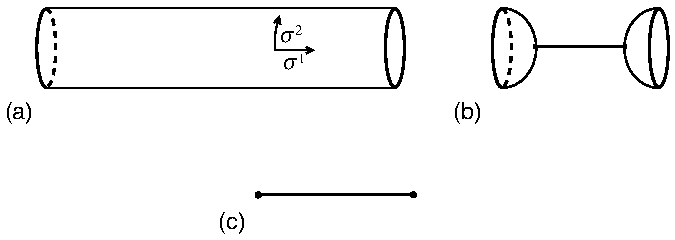
\includegraphics[width=0.8\linewidth]{figures/fig_7_1.pdf}
\caption{(a) $t$ が小さい極限の円筒。(b) 円板のタッドポール振幅と閉弦の伝播関数に分けた振幅。(c) 対応する場の理論の図。黒い丸はタッドポールを表す。}
\label{fig:7.1}
\end{figure}

円筒の $t\to\infty$ の極限は、トーラスの $\tau_2\to\infty$ の極限によく似ている。円筒は長い帯のようになり、最も軽い開弦の状態が主要な漸近挙動を与える。閉弦と同様に発散はあるが、開弦のタキオンに由来するものだけである。

$t\to0$ の極限はかなり興味深い。トーラスの場合とは異なり、積分範囲を切り取るモジュラー群の作用がないため、場の理論の UV 発散がまだ存在するように見える。しかし、弦理論のあらゆる発散と同様に、これは実際には長距離の効果として解釈すべきものであることがわかる。$t\to0$ の極限では、図\ref{fig:7.1}(a)のように円筒は非常に長くなる。つまり、閉弦が真空から現れ、ある距離を伝播してから、再び真空へ消えるように見える。このことを明確にするため、モジュラー変換(7.2.44)
\begin{equation}
\eta(it)=t^{-1/2}\eta(i/t)
\tag{7.4.2}\label{eq:7.4.2}
\end{equation}
を用い、変数を $s=\pi/t$ に変えると、
\begin{equation}
Z_{C_2}=i\frac{V_{26}n^2}{2\pi(8\pi^2\alpha')^{13}}
\int_0^\infty ds\,\eta(is/\pi)^{-24}
\tag{7.4.3}\label{eq:7.4.3}
\end{equation}
を得る。計量のスケールを $1/t$ 倍に変え、円筒の周長を通常の閉弦の周長 $2\pi$ にすると、円筒の長さは $s$ となる。
\begin{equation}
\begin{aligned}
\eta(is/\pi)^{-24}
&=\exp(2s)\prod_{n=1}^{\infty}[1-\exp(-2ns)]^{-24}\\
&=\exp(2s)+24+O(\exp(-2s))
\end{aligned}
\tag{7.4.4}\label{eq:7.4.4}
\end{equation}
と展開すると、閉弦の状態の完全系で展開したときに期待される漸近挙動が見える。言い換えると、$\sigma^2$ を世界面の時間、$\sigma^1$ を世界面の空間と考えれば、図\ref{fig:7.1}(a)は非常に短い開弦のループである。世界面の空間と時間の役割を交換すれば、境界ループから始まり、境界ループで終わる、非常に長い閉弦の世界線になる。Euclid 経路積分ではどちらの記述も使え、それぞれがモジュライ空間の異なる極限で役に立つ。

真空振幅の主要な発散は、閉弦のタキオンから生じる。これは興味の対象ではなく、解析接続によって定義できる。
\begin{equation}
\int_0^\infty ds\,\exp(\beta s)\equiv-\frac1\beta.
\tag{7.4.5}\label{eq:7.4.5}
\end{equation}
質量ゼロの閉弦の状態による第二項は、解析接続を行っても $1/0$ の形の発散を与える。この発散の起源を見るため、図\ref{fig:7.1}(b)のように過程を分けることを考えよう。第6.6節で議論したように、円板上に閉弦の頂点演算子を一つ持つ、ゼロでない振幅が存在する。このタッドポールは、閉弦が真空から現れること、あるいは真空へ消えることに対応する。二つのタッドポールの間には、閉弦の伝播関数がある。運動量空間では、質量ゼロの伝播関数は $1/k^2$ に比例する。ここでは運動量保存により、閉弦はゼロ運動量で真空から現れなければならず、そのため伝播関数は発散する。

同じ種類の発散は場の量子論にも現れる。Lagrangian に $\phi$ の一次の項を持つ、質量ゼロのスカラー場 $\phi$ を考えよう。すると、ただ一つの伝播関数につながる頂点があり、図\ref{fig:7.1}(c)の図が存在する。これは、中間の伝播関数が
\begin{equation}
\left.\frac1{k^2}\right|_{k^\mu=0}
\tag{7.4.6}\label{eq:7.4.6}
\end{equation}
であるために発散する。伝播関数の極は時空の長距離にわたる伝播と関係するので、これは長距離（IR）発散である。

場の量子論における UV 発散と IR 発散は、物理的起源が大きく異なる。UV 発散は通常、理論の破綻、ある短距離で新しい物理が必要になることを示す。IR 発散は一般に、問いの立て方が誤っているか、展開の仕方が誤っていることを意味する。ここでもそうである。通常の摂動論では、$\phi(x)=0$、あるいは他の定数の配位の周りで展開する。作用
\begin{equation}
-\frac1{g^2}\int d^dx
\left(\frac12\partial_\mu\phi\,\partial^\mu\phi+g\Lambda\phi\right)
\tag{7.4.7}\label{eq:7.4.7}
\end{equation}
に対し、運動方程式
\begin{equation}
\partial^2\phi=g\Lambda
\tag{7.4.8}\label{eq:7.4.8}
\end{equation}
は $\phi(x)=0$ を解として認めない。その代わりに、方程式\hyperref[eq:7.4.8]{(7.4.8)}の解の周りで展開しなければならない。どの解も必然的に位置に依存する。その結果得られる振幅には発散がない。右辺が摂動であるにもかかわらず（円板に適した因子 $g$ を含めてある）、こうなるのは、それが特異摂動だからである。特に、補正された背景は、ゼロ次の解の Poincaré 対称性の一部を破る。

弦理論でも状況はまったく同じである。円板のタッドポールは、ディラトンと計量の両方に対する源
\begin{equation}
-\Lambda\int d^{26}x\,(-G)^{1/2}e^{-\tilde\Phi}
\tag{7.4.9}\label{eq:7.4.9}
\end{equation}
となる。補正された場の方程式の解の周りで（計量とディラトンはもはや定数ではない）展開すれば、有限な振幅が得られる。詳細はやや複雑なので、第9章でもう少し議論する。なお、超対称な弦理論では、ツリーレベルの背景が超対称性のもとで不変であれば、通常はループ補正を受けない。

極\hyperref[eq:7.4.6]{(7.4.6)}は、ツリーレベルの振幅で出会ったものと同じ種類の発散、すなわち時空の長距離にわたる伝播に対応する共鳴である。円筒の両端に開弦の頂点演算子を加え、1ループの開弦散乱振幅を表すようにすると、一方の境界から他方へ流れる運動量 $k^\mu$ は一般にゼロでなくなる。このとき、大きい $s$ の極限\hyperref[eq:7.4.4]{(7.4.4)}には因子
\begin{equation}
\exp(-\alpha'k^2s/2)
\tag{7.4.10}\label{eq:7.4.10}
\end{equation}
が含まれ、発散は、開弦が中間状態の閉弦へ散乱することを表す運動量の極になる。したがって、第3章で述べたように、開弦理論は閉弦も含まなければならない。UV 発散を除く機構が、閉弦と開弦で異なるのは興味深い。閉弦ではモジュライ積分に対する実効的なカットオフであり、開弦では、モジュライ空間の危険な極限を長距離の現象として解釈し直すことである。

式\hyperref[eq:7.4.1]{(7.4.1)}では、$\sigma^2$ を時間として経路積分を切り開き、円筒上の経路積分を開弦のスペクトルについてのトレースに関係づけた。$\sigma^1$ を時間とすれば、閉弦の Hilbert 空間を用いて得ることもできる。$\sigma^2$ の周期を $2\pi$ とし、境界を $\sigma^1=0,s$ に置こう。閉弦は $\sigma^1=0$ である状態 $\lvert B\rangle$ として現れ、$\sigma^1=s$ で同じように消える。測度に伴う挿入を含めると、経路積分は
\begin{equation}
\langle B|c_0b_0\exp[-s(L_0+\tilde L_0)]|B\rangle
\tag{7.4.11}\label{eq:7.4.11}
\end{equation}
に比例する。境界状態 $\lvert B\rangle$ は、$\partial_1X^\mu,c^1,b_{12}$ が境界で消えるという条件で定まる。Hamiltonian 形式では、これらは $\lvert B\rangle$ を消さなければならない。Laurent 係数で書けば、
\begin{equation}
\begin{aligned}
(\alpha_n^\mu+\tilde\alpha_{-n}^\mu)|B\rangle
&=(c_n+\tilde c_{-n})|B\rangle\\
&=(b_n-\tilde b_{-n})|B\rangle=0,
\qquad\text{すべての }n
\end{aligned}
\tag{7.4.12}\label{eq:7.4.12}
\end{equation}
である。これによって
\begin{equation}
\begin{aligned}
|B\rangle\propto{}&(c_0+\tilde c_0)\\
&\times\exp\left[-\sum_{n=1}^{\infty}
\left(n^{-1}\alpha_{-n}\cdot\tilde\alpha_{-n}
+b_{-n}\tilde c_{-n}+\tilde b_{-n}c_{-n}\right)\right]|0;0\rangle
\end{aligned}
\tag{7.4.13}\label{eq:7.4.13}
\end{equation}
と定まる。これを\hyperref[eq:7.4.11]{(7.4.11)}に用いると、$\lvert B\rangle$ の規格化が未定であることを除いて、結果\hyperref[eq:7.4.3]{(7.4.3)}を得る。この表示は $t\to0$ の極限と閉弦の極を解析するのに有用である。

弦と場の理論の計算を比較することで、円板のタッドポール $\Lambda$ を決められる。ただし、次章で、より一般的な結果の特殊例として求める方が便利である。

\subsubsectionlink*{Klein の壺}

Klein の壺からの真空振幅は
\begin{equation}
\begin{aligned}
Z_{K_2}
&=\int_0^\infty\frac{dt}{4t}\operatorname{Tr}'_{\mathrm c}
\left\{\Omega\exp[-2\pi t(L_0+\tilde L_0)]\right\}\\
&=iV_d\int_0^\infty\frac{dt}{4t}(4\pi^2\alpha't)^{-d/2}
\sum_{i\in\mathcal H_{\mathrm c}^\perp}
\Omega_i\exp[-2\pi t(h_i+\tilde h_i-2)]
\end{aligned}
\tag{7.4.14}\label{eq:7.4.14}
\end{equation}
であり、記法は円筒の式\hyperref[eq:7.4.1]{(7.4.1)}に従う。向き付けのある理論のトーラスに比べ、射影演算子 $\tfrac12(1+\Omega)$ に由来する因子 $\tfrac12$ が余分にある。同じ理由で、向き付けのない理論では、トーラスと円筒の両方の振幅に余分な $\tfrac12$ が付く。これは、追加のゲージ不変性 $w\to\bar w$ に由来すると考えてもよい。平坦な26次元でトレースを評価するには、$\Omega$ の対角要素は、右向きと左向きが同じ状態にあるものだけであり、これらは $\Omega=+1$ で寄与することに注意する。するとトレースは実効的に片側だけにわたり、開弦のスペクトルと同じになる。ただし、右向きと左向きが等しい寄与をするため、共形ウェイトは二倍になる。結果は
\begin{equation}
Z_{K_2}\longrightarrow iV_{26}\int_0^\infty\frac{dt}{4t}
(4\pi^2\alpha't)^{-13}\eta(2it)^{-24}
\tag{7.4.15}\label{eq:7.4.15}
\end{equation}
である。

\begin{figure}[tbp]
\centering
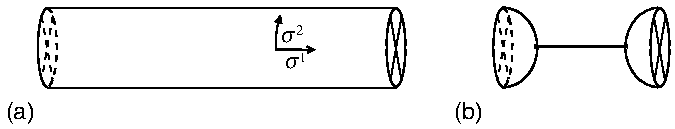
\includegraphics[width=0.8\linewidth]{figures/fig_7_2.pdf}
\caption{(a) $t$ が小さい極限の Klein の壺を、クロスキャップで両端をふさいだ円筒として表したもの。(b) $RP_2$ のタッドポール振幅と閉弦の伝播関数に分けた振幅。}
\label{fig:7.2}
\end{figure}

モジュラス $t$ は円筒と同じ範囲 $0<t<\infty$ を動くので、$t\to0$ の発散も同じである。ここでも $1/0$ の極は、閉弦の極として長距離の解釈を持つ。これを見るため、領域
\begin{align}
0\leq\sigma^1\leq2\pi,\qquad&0\leq\sigma^2\leq2\pi t,
\tag{7.4.16a}\label{eq:7.4.16a}\\
0\leq\sigma^1\leq\pi,\qquad&0\leq\sigma^2\leq4\pi t
\tag{7.4.16b}\label{eq:7.4.16b}
\end{align}
を考えよう。どちらも同一視
\begin{equation}
w\cong w+2\pi\cong-\bar w+2\pi it
\tag{7.4.17}\label{eq:7.4.17}
\end{equation}
の基本領域である。\hyperref[eq:7.4.16a]{(7.4.16a)}では、左右の辺が周期的に同一視され、上下の辺はパリティ反転の後に同一視されるため、$\Omega$ で重みを付けた閉弦のループとして解釈できる。\hyperref[eq:7.4.16b]{(7.4.16b)}については、同一視\hyperref[eq:7.4.17]{(7.4.17)}から
\begin{equation}
w\cong w+4\pi it,\qquad
w+\pi\cong-(\bar w+\pi)+2\pi it
\tag{7.4.18}\label{eq:7.4.18}
\end{equation}
も従うことに注意しよう。これより、領域\hyperref[eq:7.4.16b]{(7.4.16b)}の上下の辺は周期的に同一視される。左辺は、その長さの半分だけ平行移動し、辺に関して反射した後の自分自身と同一視される。右辺も同様であり、これはクロスキャップの定義である。したがって、図\ref{fig:7.2}(a)のように、二つのクロスキャップで両端をふさいだ円筒という表示が得られる。$1/(2t)$ 倍にスケールを変えると、円筒の周長は $2\pi$、長さは $s=\pi/(2t)$ になる。モジュラー変換の後、振幅は
\begin{equation}
Z_{K_2}=i\frac{2^{26}V_{26}}{4\pi(8\pi^2\alpha')^{13}}
\int_0^\infty ds\,\eta(is/\pi)^{-24}
\tag{7.4.19}\label{eq:7.4.19}
\end{equation}
となる。タッドポールが円板ではなく射影平面から生じることを除けば、円筒の発散についての議論がすべて当てはまる。

\subsubsectionlink*{Möbius の帯}

Möbius の帯については、
\begin{equation}
Z_{M_2}=iV_d\int_0^\infty\frac{dt}{4t}
(8\pi^2\alpha't)^{-d/2}
\sum_{i\in\mathcal H_{\mathrm o}^\perp}
\Omega_i\exp[-2\pi t(h_i-1)].
\tag{7.4.20}\label{eq:7.4.20}
\end{equation}
これは、$\Omega$ と、射影演算子に由来する因子 $\tfrac12$ だけが円筒の結果と異なる。平坦な26次元では、トレース中の演算子 $\Omega$ の効果は、偶数の質量レベルに余分な $-1$ を付け、Chan--Paton 因子を適切に数えることである。したがって、振動子のトレースは
\begin{equation}
\exp(2\pi t)\prod_{n=1}^{\infty}
[1-(-1)^n\exp(-2\pi nt)]^{-24}
=\vartheta_{00}(0,2it)^{-12}\eta(2it)^{-12}
\tag{7.4.21}\label{eq:7.4.21}
\end{equation}
となる。$SO(n)$ 理論では、$\tfrac12n(n+1)$ 個の対称な状態は $\Omega=+1$、$\tfrac12n(n-1)$ 個の反対称な状態は $\Omega=-1$ を持つので、正味の寄与は $n$ である。$Sp(k)$ 理論では、これらの縮退度が逆になり、$-n$ を与える（ここでの記法では、$Sp(k)$ は $n=2k$ 個の Chan--Paton 状態に対応することを思い出そう）。すると振幅は
\begin{equation}
Z_{M_2}=\pm inV_{26}\int_0^\infty\frac{dt}{4t}
(8\pi^2\alpha't)^{-13}
\vartheta_{00}(0,2it)^{-12}\eta(2it)^{-12}
\tag{7.4.22}\label{eq:7.4.22}
\end{equation}
である。

\begin{figure}[tbp]
\centering
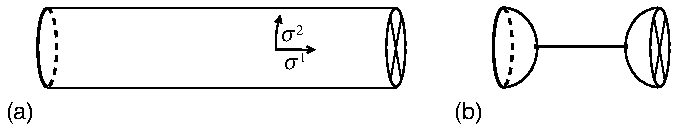
\includegraphics[width=0.8\linewidth]{figures/fig_7_3.pdf}
\caption{(a) $t$ が小さい極限の Möbius の帯を、クロスキャップを一つ付けた円筒として表したもの。(b) $D_2$ と $RP_2$ のタッドポール振幅、および閉弦の伝播関数に分けた振幅。}
\label{fig:7.3}
\end{figure}

Klein の壺と同じ構成により、Möbius の帯は、図\ref{fig:7.3}(a)のように、一端が境界で他端がクロスキャップである円筒として表せる。今度の円筒の長さは $s=\pi/(4t)$ である。モジュラー変換により、振幅は
\begin{equation}
Z_{M_2}=\pm2in\frac{2^{13}V_{26}}{4\pi(8\pi^2\alpha')^{13}}
\int_0^\infty ds\,\vartheta_{00}(0,2is/\pi)^{-12}
\eta(2is/\pi)^{-12}
\tag{7.4.23}\label{eq:7.4.23}
\end{equation}
となる。環帯の場合と同じく、これも演算子による表式に書ける。式\hyperref[eq:7.4.11]{(7.4.11)}の境界状態の一つを、同様のクロスキャップ状態 $\lvert C\rangle$ に置き換えればよい。ここでも $t\to0$ の発散があり、円板から一つ、射影平面から一つのタッドポールが生じる、図\ref{fig:7.3}(a)の過程に対応する。

向き付けのない理論では、これら三つの曲面の発散が合わさって
\begin{equation}
i\frac{24V_{26}}{4\pi(8\pi^2\alpha')^{13}}
(2^{13}\mp n)^2\int_0^\infty ds
\tag{7.4.24}\label{eq:7.4.24}
\end{equation}
となる。すなわち、全タッドポールは $2^{13}\mp n$ に比例する。ゲージ群 $SO(2^{13})=SO(8192)$ では、円板と射影平面のタッドポールが相殺して、これはゼロになる。ボソン弦ではおそらく特別な意味を持たないが、超弦理論における $SO(32)$ の同様の相殺には特別な意味がある。

\subsectionlink*{演習}
\addcontentsline{toc}{subsection}{第7章の演習}

\subsubsection*{演習7.1}\label{ex:7.1}
トーラス上の指数演算子の期待値\hyperref[eq:7.2.4]{(7.2.4)}に至る手順を補え。$\tau\to-1/\tau$ のもとで正しく変換することを示せ。

\subsubsection*{演習7.2}\label{ex:7.2}
付録Aで調和演算子について行うように、行列式を正則化して評価することにより、トーラスの真空振幅\hyperref[eq:7.3.6]{(7.3.6)}を導け。モジュラー変換が固有値を置換するだけであることを示せ。［演習A.3と比較せよ。］（参考文献：Polchinski (1986)。）

\subsubsection*{演習7.3}\label{ex:7.3}
固有関数の和(6.2.7)を実行して、Green 関数\hyperref[eq:7.2.3]{(7.2.3)}を導け。

\subsubsection*{演習7.4}\label{ex:7.4}
トーラス上の $\langle\partial_wX^\mu(w)\partial_wX_\mu(0)\rangle$ を、トレースとして表すことによって評価せよ。結果が式\hyperref[eq:7.2.16]{(7.2.16)}と一致することを示せ。

\subsubsection*{演習7.5}\label{ex:7.5}
\begin{enumerate}
\item[(a)] $\operatorname{Im}\tau\to\infty$ におけるテータ関数(7.2.37)の主要な挙動を求めよ。
\item[(b)] モジュラー変換を用い、虚軸に沿って $\tau\to0$ とするときについても同じことを行え。
\item[(c)] より風変わりな問いとして、$\tau$ が虚軸に平行な経路に沿って実軸上のゼロでない点に近づくときはどうなるか。［ヒント：その点が有理数か無理数かによって、答えは本質的に異なる。］
\end{enumerate}

\subsubsection*{演習7.6}\label{ex:7.6}
\begin{enumerate}
\item[(a)] 式\hyperref[eq:7.3.20]{(7.3.20)}、\hyperref[eq:7.3.21]{(7.3.21)}を確かめよ。
\item[(b)] 任意の次元 $d$ で、$l$ 積分にカットオフを課して $Z_{S_1}(m^2)$ を評価せよ。相殺項が $m^2$ に関して解析的であることを示せ。$d=4$ における非解析的な部分を与えよ。（参考文献：Coleman \& Weinberg (1973)。）
\end{enumerate}

\subsubsection*{演習7.7}\label{ex:7.7}
円筒上の $n$ 個の開弦タキオンの振幅を、トーラスの振幅（式\hyperref[eq:7.3.6]{(7.3.6)}と式\hyperref[eq:7.2.4]{(7.2.4)}を組み合わせたもの）と同様の形で求めよ。必要な Green 関数は、円筒をトーラスの対合として表す表示を用い、鏡像法によってトーラス上の Green 関数から得られる。

\subsubsection*{演習7.8}\label{ex:7.8}
二つの境界のそれぞれにいくつかの頂点演算子がある場合について、前問の振幅を考えよ。前問の具体的な結果から、$t\to0$ の極限が、一方の境界から他方へ流れる運動量の関数として、閉弦の極の列を与えることを示せ。

\subsubsection*{演習7.9}\label{ex:7.9}
演習6.12と7.8の両方を解いた場合、ユニタリ性が、前者の二乗を後者のタキオンの極に関係づけることを論じよ。これを用いて $g_{\mathrm c}$ と $g_{\mathrm o}^2$ の数値的な関係を求めよ。次章では、これと似たことを、より回り道をして行う。

\subsubsection*{演習7.10}\label{ex:7.10}
中間状態の開弦に関する円筒振幅のユニタリ性が、Chan--Paton 因子に
\[
\operatorname{Tr}(\lambda^a\lambda^b)\operatorname{Tr}(\lambda^c\lambda^d)
=\operatorname{Tr}(\lambda^a\lambda^b\lambda^e\lambda^c\lambda^d\lambda^e)
\]
を要求することを論じよ。ゲージ群 $U(n_1)\times U(n_2)\times\cdots\times U(n_k)$ はツリーレベルのユニタリ性と整合するが、この追加の条件は $U(n)$ を選び出すことを示せ。

\subsubsection*{演習7.11}\label{ex:7.11}
この演習は、弦理論における $D=26$ の最初の出現（Lovelace, 1971）を再現する。時空の次元を $D$、正味の振動子の組の数を $D'$ と仮定し、\hyperref[eq:7.3.9]{(7.3.9)}の形の Coleman--Weinberg 公式から円筒の真空振幅を計算せよ。頂点演算子の共形不変性が要求するとおり、タキオンの質量を $m^2=-1/\alpha'$ に保つように、開弦の質量二乗の定数項を定めよ。散乱振幅を模擬するため、式\hyperref[eq:7.4.10]{(7.4.10)}のように因子 $\exp(-\alpha'k^2s/2)$ を追加せよ。$D=26$ かつ $D'=24$ でない限り、振幅が $k^2$ に関して極ではなく分岐切断を持つことを示せ。

\subsubsection*{演習7.12}\label{ex:7.12}
前問をトーラスについて繰り返し、この場合には $D=26$ かつ $D'=24$ のときに限り、真空振幅がモジュラー不変であることを示せ（Shapiro, 1972）。

\subsubsection*{演習7.13}\label{ex:7.13}
トーラスの振幅\hyperref[eq:7.3.6]{(7.3.6)}の導出と同様の手順を実行し、弦の経路積分から Klein の壺の真空振幅\hyperref[eq:7.4.15]{(7.4.15)}を求めよ。

\subsubsection*{演習7.14}\label{ex:7.14}
境界状態\hyperref[eq:7.4.13]{(7.4.13)}を用いた振幅\hyperref[eq:7.4.11]{(7.4.11)}が、円筒の振幅\hyperref[eq:7.4.3]{(7.4.3)}を再現することを示せ。

\subsubsection*{演習7.15}\label{ex:7.15}
\begin{enumerate}
\item[(a)] クロスキャップに対応する状態 $\lvert C\rangle$ を求めよ。
\item[(b)] 式\hyperref[eq:7.4.11]{(7.4.11)}に類似した式によって、Klein の壺と Möbius の帯の真空振幅を求めよ。
\end{enumerate}
